\noindent
\begin{minipage}{\linewidth}
    \centering
    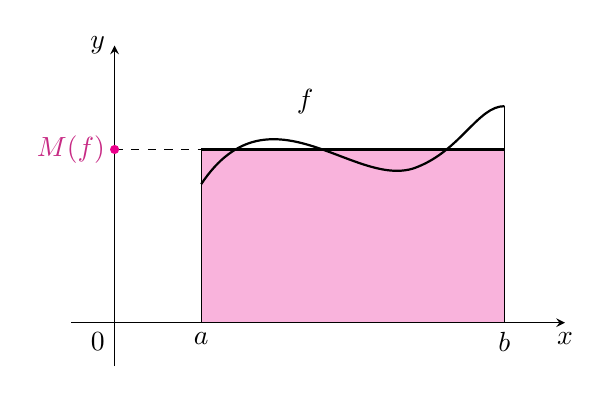
\begin{tikzpicture}[>=stealth, scale=1.1]
        \fill[magenta!30] (1,0) rectangle (4.5, 2.0);
        \draw[->] (-0.5,0) -- (5.2,0) node[below] {$x$};
        \draw[->] (0,-0.5) -- (0,3.2) node[left] {$y$};
        \draw (1,0) -- (1, 2.0);
        \draw (4.5,0) -- (4.5, 2.5);
        \draw[thick] (1, 2.0) -- (4.5, 2.0);
        \draw[dashed] (0, 2.0) -- (1, 2.0);
        \draw[thick] (1, 1.6) 
            .. controls (1.8, 2.8) and (2.8, 1.5) .. (3.5, 1.8)
            .. controls (4.0, 2.0) and (4.2, 2.5) .. (4.5, 2.5);
        \node[below left] at (0,0) {$0$};
        \node[below] at (1,0) {$a$};
        \node[below] at (4.5,0) {$b$};
        \node[left, color=magenta!80!black] at (0,2.0) {$M(f)$};
        \node[above] at (2.2, 2.3) {$f$};
        \fill[magenta] (0,2.0) circle (1.5pt);
    \end{tikzpicture}
\end{minipage}

\vspace{5pt}
\noindent \textbf{Рис. 3.}

\vspace{10pt}

\noindent
\textbf{Упражнение 5.} Докажите, что если $a, b, c, d$ --- действительные числа, сумма которых равна 0, то
\begin{equation}
|a| + |b| + |c| + |d| \ge |a+d| + |b+d| + |c+d|. \tag{4}
\end{equation}

\noindent
\textbf{Решение.} Если в (3) векторы $\vec{a}, \vec{b}, \vec{c}, \vec{d}$ заменить их проекциями на какую-нибудь ось («Геометрия 9»), получится (4). Возникает идея: доказать (3), рассматривая проекции данных векторов $\vec{a}, \vec{b}, \vec{c}, \vec{d}$ на всевозможные оси. Попробуем ее реализовать.

Пусть $\vec{p}$ --- вектор. Введем вспомогательную функцию $p$ следующим образом: фиксируем некоторую ось $l_0$; обозначим через $p(\alpha)$ проекцию вектора $\vec{p}$ на ось $l$, образующую с осью $l_0$ угол $\alpha$ (рис. 4). Если $\varphi$ --- угол между вектором $\vec{p}$ и осью $l_0$, то $p(\alpha) = |\vec{p}|\cos(\varphi - \alpha)$.

Рассмотрим среднее значение $M(|\vec{p}|)$ функции $\alpha \to |p(\alpha)|$ на отрезке $[0; 2\pi]$. Из определения (2)
\begin{align*}
M(|p|) &= \frac{1}{2\pi} \int\limits_{0}^{2\pi} |p(\alpha)|\, d\alpha = \\
&= \frac{1}{2\pi} \int\limits_{0}^{2\pi} |p| |\cos(\varphi - \alpha)|\, d\alpha = \\
&= \frac{|\vec{p}|}{2\pi} \int\limits_{0}^{2\pi} |\cos(\varphi - \alpha)|\, d\alpha. \tag{5}
\end{align*}

Покажем существование такого $k \neq 0$, что для любого вектора $\vec{p}$ справедливо равенство
\begin{equation}
M(|p|) = k\, |\vec{p}|. \tag{6}
\end{equation}

\vspace{\fill}
\newpage 

\noindent
\begin{minipage}{\linewidth}
    \centering
    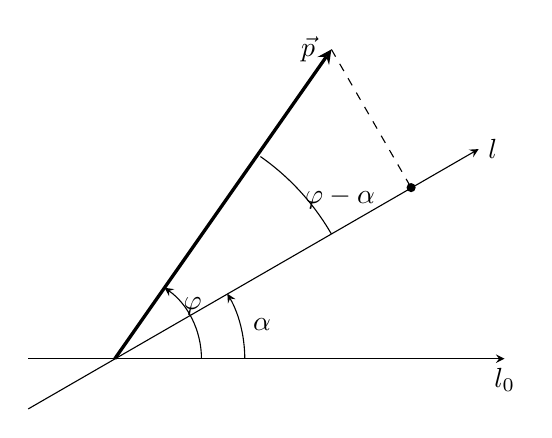
\begin{tikzpicture}[>=stealth, scale=1.1]
        \coordinate (O) at (0,0);
        \draw[->] (-1,0) -- (4.5,0) node[below] {$l_0$};
        \draw[->] (-1, -0.58) -- (4.2, 2.42) node[right] {$l$};
        \draw[->, very thick] (O) -- (2.5, 3.57) node[left, xshift=-2pt] {$\vec{p}$};
        \coordinate (P) at (2.5, 3.57);
        \coordinate (Proj) at (3.42, 1.975);
        \draw[dashed] (P) -- (Proj);
        \fill (Proj) circle (1.5pt);
        \draw[->] (1.5,0) arc (0:30:1.5);
        \node at (1.7, 0.4) {$\alpha$};
        \draw[->] (1.0,0) arc (0:55:1.0);
        \node at (0.9, 0.6) {$\varphi$};
        \draw (2.5, 1.44) arc (30:55:2.8);
        \node at (2.6, 1.85) {$\varphi - \alpha$};
    \end{tikzpicture}
\end{minipage}

\vspace{5pt}
\noindent \textbf{Рис. 4.}

\vspace{10pt}

\noindent
В силу (5) достаточно доказать, что интеграл $\displaystyle \int\limits_{0}^{2\pi} |\cos(\varphi - \alpha)|\, d\alpha$ не зависит от вектора $\vec{p}$, то есть не зависит от угла $\varphi$.
\begin{align*}
\int\limits_{0}^{2\pi} & |\cos(\varphi - \alpha)|\, d\alpha = \int\limits_{0}^{2\pi} |\cos(\alpha - \varphi)|\, d\alpha = \\
&= \int\limits_{0-\varphi}^{2\pi-\varphi} |\cos \alpha|\, d\alpha = \int\limits_{-\varphi}^{2\pi-\varphi} |\cos \alpha|\, d\alpha = \\
&= \int\limits_{-\varphi}^{0} |\cos \alpha|\, d\alpha + \int\limits_{0}^{2\pi-\varphi} |\cos \alpha|\, d\alpha = \\
&= \int\limits_{2\pi-\varphi}^{2\pi} |\cos(\alpha - 2\pi)|\, d\alpha + \\
&+ \int\limits_{0}^{2\pi-\varphi} |\cos \alpha|\, d\alpha = \int\limits_{2\pi-\varphi}^{2\pi} |\cos \alpha|\, d\alpha + \\
&+ \int\limits_{0}^{2\pi-\varphi} |\cos \alpha|\, d\alpha = \int\limits_{0}^{2\pi-\varphi} |\cos \alpha|\, d\alpha + \\
&+ \int\limits_{2\pi-\varphi}^{2\pi} |\cos \alpha|\, d\alpha = \int\limits_{0}^{2\pi} |\cos \alpha|\, d\alpha. \tag{7}
\end{align*}

\vspace{1em}
В этой выкладке использованы два свойства интегралов:
\begin{equation*}
\int\limits_{a}^{b} f(x+p)\, dx = \int\limits_{a+p}^{b+p} f(x)\, dx,
\end{equation*}
\begin{equation*}
\int\limits_{a}^{b} f(x)\, dx = \int\limits_{a}^{c} f(x)\, dx + \int\limits_{c}^{b} f(x)\, dx
\end{equation*}

\vspace{\fill}
\noindent